\documentclass{article}
\usepackage{amsfonts}
\usepackage{amsmath}
\usepackage{amssymb}
\usepackage{amsthm}
\usepackage{graphicx} % Required for inserting images
\usepackage{listings}
\usepackage{xcolor}
\usepackage{caption}
\usepackage{subcaption}
\usepackage{float}
%custom colors
\definecolor{codegray}{rgb}{0.5,0.5,0.5}
\definecolor{codeblue}{rgb}{0.25,0.5,0.75}
\definecolor{codepurple}{rgb}{0.58,0,0.82}

% Configure listings
\lstset{
    language=Python,
    basicstyle=\ttfamily\small,
    keywordstyle=\color{codeblue}\bfseries,
    commentstyle=\color{codegray}\itshape,
    stringstyle=\color{codepurple},
    showstringspaces=false,
    numbers=left,
    numberstyle=\tiny\color{codegray},
    frame=single,
    breaklines=true,
    captionpos=b,
    morekeywords={self}  % Add keywords here
}

\newcommand{\imgwidth}{0.45\textwidth}

\title{AI 539 \\ Homework 4}
\author{Ameyassh Nagarajan}
\date{June 2024}

\begin{document}

\maketitle

\section{Section 1}
\subsection{Task 1.1}

To achieve \( a \approx v_j \), the dot product \( q \cdot k_j \) must be significantly larger than \( q \cdot k_i \) for all \( i \neq j \). This ensures that the attention weight \( \alpha_j \) corresponding to \( v_j \) is close to 1, while the other weights are close to 0. Therefore, the query \( q \) must be closely aligned with the key \( k_j \).

\subsection{Task 1.2}
Given that the keys are orthogonal unit vectors, we can construct a query vector \( q \) that is equidistant from \( k_a \) and \( k_b \). A simple way to achieve this is to take the sum of \( k_a \) and \( k_b \):

\[
q = k_a + k_b
\]

The dot products for this query vector are:

\[
q \cdot k_a = (k_a + k_b) \cdot k_a = 1 + 0 = 1
\]
\[
q \cdot k_b = (k_a + k_b) \cdot k_b = 0 + 1 = 1
\]

For any other key \( k_i \) orthogonal to \( k_a \) and \( k_b \):

\[
q \cdot k_i = (k_a + k_b) \cdot k_i = 0 + 0 = 0
\]

The softmax function will assign equal weights to \( k_a \) and \( k_b \) and a much smaller weight to all other keys. Hence, the attention weights will be approximately:

\[
\alpha_a \approx \frac{1}{2}, \quad \alpha_b \approx \frac{1}{2}, \quad \alpha_i \approx 0 \quad \text{for all } i \neq a, b
\]

Therefore, the output will be:

\[
a \approx \alpha_a v_a + \alpha_b v_b = \frac{1}{2} v_a + \frac{1}{2} v_b = \frac{1}{2} (v_a + v_b)
\]

\subsection{Task 1.3}
Given the query vector \( q = \mu_a + \mu_b \):

1. For \( k_a \):
   \[
   q \cdot k_a = (\mu_a + \mu_b) \cdot (\mu_a \lambda_a) = \mu_a \cdot \mu_a \lambda_a + \mu_b \cdot \mu_a \lambda_a = \lambda_a
   \]
   This is because \( \mu_a \cdot \mu_a = 1 \) and \( \mu_b \cdot \mu_a = 0 \) (due to orthogonality).

2. For \( k_b \):
   \[
   q \cdot k_b = (\mu_a + \mu_b) \cdot (\mu_b \lambda_b) = \mu_a \cdot \mu_b \lambda_b + \mu_b \cdot \mu_b \lambda_b = \lambda_b
   \]
   This is because \( \mu_b \cdot \mu_b = 1 \) and \( \mu_a \cdot \mu_b = 0 \) (due to orthogonality).

For any other key \( k_i \) orthogonal to \( \mu_a \) and \( \mu_b \):
   \[
   q \cdot k_i = (\mu_a + \mu_b) \cdot (\mu_i \lambda_i) = \mu_a \cdot \mu_i \lambda_i + \mu_b \cdot \mu_i \lambda_i = 0
   \]
   This is because \( \mu_a \cdot \mu_i = 0 \) and \( \mu_b \cdot \mu_i = 0 \) (due to orthogonality).

The attention weights are computed using the softmax function:
   \[
   \alpha_i = \frac{\exp(q \cdot k_i / \sqrt{d})}{\sum_{j=1}^{m} \exp(q \cdot k_j / \sqrt{d})}
   \]

For \( k_a \) and \( k_b \), the dot products are \(\lambda_a\) and \(\lambda_b\), respectively. Thus, the attention weights \(\alpha_a\) and \(\alpha_b\) are:
   \[
   \alpha_a \approx \frac{\exp(\lambda_a / \sqrt{d})}{\exp(\lambda_a / \sqrt{d}) + \exp(\lambda_b / \sqrt{d})}
   \]
   \[
   \alpha_b \approx \frac{\exp(\lambda_b / \sqrt{d})}{\exp(\lambda_a / \sqrt{d}) + \exp(\lambda_b / \sqrt{d})}
   \]

Since \(\lambda_i \sim \mathcal{N}(1, \beta)\), the values of \(\lambda_a\) and \(\lambda_b\) will fluctuate due to the random sampling. This means the attention weights \(\alpha_a\) and \(\alpha_b\) will also fluctuate, causing variability in the output \(a\).

Over multiple resamplings of \(\lambda_1, ..., \lambda_m\), the output \(a\) will vary due to the fluctuations in the attention weights. However, because \(\lambda_i\) values are sampled from a normal distribution centered around 1, the fluctuations will average out over many resamplings. This means that on average, the output \(a\) will be approximately:
   \[
   a \approx \frac{1}{2}(v_a + v_b)
   \]
But individual outputs will show variation due to the noise introduced by the \(\lambda\)'s.

\subsection{Task 1.4}
In Task 1.2, we designed a query \( q \) that would lead to the output being an average of \( v_a \) and \( v_b \). For multi-head attention, we need to design two queries \( q_1 \) and \( q_2 \) that will result in \( a_1 \) and \( a_2 \) being close to \( v_a \) and \( v_b \), and their average should be close to \( \frac{1}{2}(v_a + v_b) \).

Given the orthogonal unit vectors \( \mu_i \) and the noisy scaling factors \( \lambda_i \), we can construct the queries as follows:

1. First query \( q_1 \) should be the sum of \( \mu_a \) and \( \mu_b \):
   \[
   q_1 = \mu_a + \mu_b
   \]

2. Second query \( q_2 \) should be the difference of \( \mu_a \) and \( \mu_b \):
   \[
   q_2 = \mu_a - \mu_b
   \]

For \( q_1 \):
   \[
   q_1 \cdot k_a = (\mu_a + \mu_b) \cdot (\mu_a \lambda_a) = \lambda_a
   \]
   \[
   q_1 \cdot k_b = (\mu_a + \mu_b) \cdot (\mu_b \lambda_b) = \lambda_b
   \]

For \( q_2 \):
   \[
   q_2 \cdot k_a = (\mu_a - \mu_b) \cdot (\mu_a \lambda_a) = \lambda_a
   \]
   \[
   q_2 \cdot k_b = (\mu_a - \mu_b) \cdot (\mu_b \lambda_b) = -\lambda_b
   \]

The attention weights for each head will fluctuate due to the noise introduced by the \( \lambda \)'s, but the combination of both heads should average out the noise to some extent.

The outputs for the heads will be:
   \[
   a_1 \approx \frac{1}{2}(v_a + v_b)
   \]
   \[
   a_2 \approx \frac{1}{2}(v_a - v_b)
   \]

Combining these:
   \[
   a = \frac{1}{2}(a_1 + a_2) \approx \frac{1}{2} \left( \frac{1}{2}(v_a + v_b) + \frac{1}{2}(v_a - v_b) \right) = \frac{1}{2} \left( v_a + \frac{v_a - v_b}{2} \right) = \frac{1}{2}(v_a + v_b)
   \]

Thus, the queries \( q_1 \) and \( q_2 \) designed as \( q_1 = \mu_a + \mu_b \) and \( q_2 = \mu_a - \mu_b \) will result in the final output being approximately \( \frac{1}{2}(v_a + v_b) \).

\pagebreak
\section{Section 2}
\subsection{Task 2.1}
Here is the implementation of the \texttt{SingleQueryScaledDotProductAttention} class in Python:

\begin{lstlisting}[caption={SingleQueryScaledDotProductAttention Class}, label={lst:scaled_dot_product}]
import torch
import torch.nn as nn
import torch.nn.functional as F

class SingleQueryScaledDotProductAttention(nn.Module):
    def __init__(self, enc_hid_dim, dec_hid_dim, kq_dim=64):
        super().__init__()
        self.q_proj = nn.Linear(dec_hid_dim, kq_dim)
        self.k_proj = nn.Linear(enc_hid_dim * 2, kq_dim)
        self.v_proj = nn.Linear(enc_hid_dim * 2, enc_hid_dim * 2)
        self.scale = torch.sqrt(torch.FloatTensor([kq_dim])).to(torch.device("cuda" if torch.cuda.is_available() else "cpu"))

    def forward(self, hidden, encoder_outputs):
        queries = self.q_proj(hidden).unsqueeze(1)  # [batch_size, 1, kq_dim]
        keys = self.k_proj(encoder_outputs)  # [batch_size, src_len, kq_dim]
        values = self.v_proj(encoder_outputs)  # [batch_size, src_len, enc_hid_dim * 2]

        # Compute the dot products
        energy = torch.bmm(queries, keys.transpose(1, 2)) / self.scale  # [batch_size, 1, src_len]
        alpha = F.softmax(energy, dim=-1)  # [batch_size, 1, src_len]

        # Compute the weighted sum of values
        attended_val = torch.bmm(alpha, values).squeeze(1)  # [batch_size, enc_hid_dim * 2]

        return attended_val, alpha.squeeze(1)
\end{lstlisting}

\pagebreak

\subsection*{TASK 2.2 Attention Diagrams}

\subsubsection*{Attention Diagram Examples}

\begin{figure}[H]
    \centering
    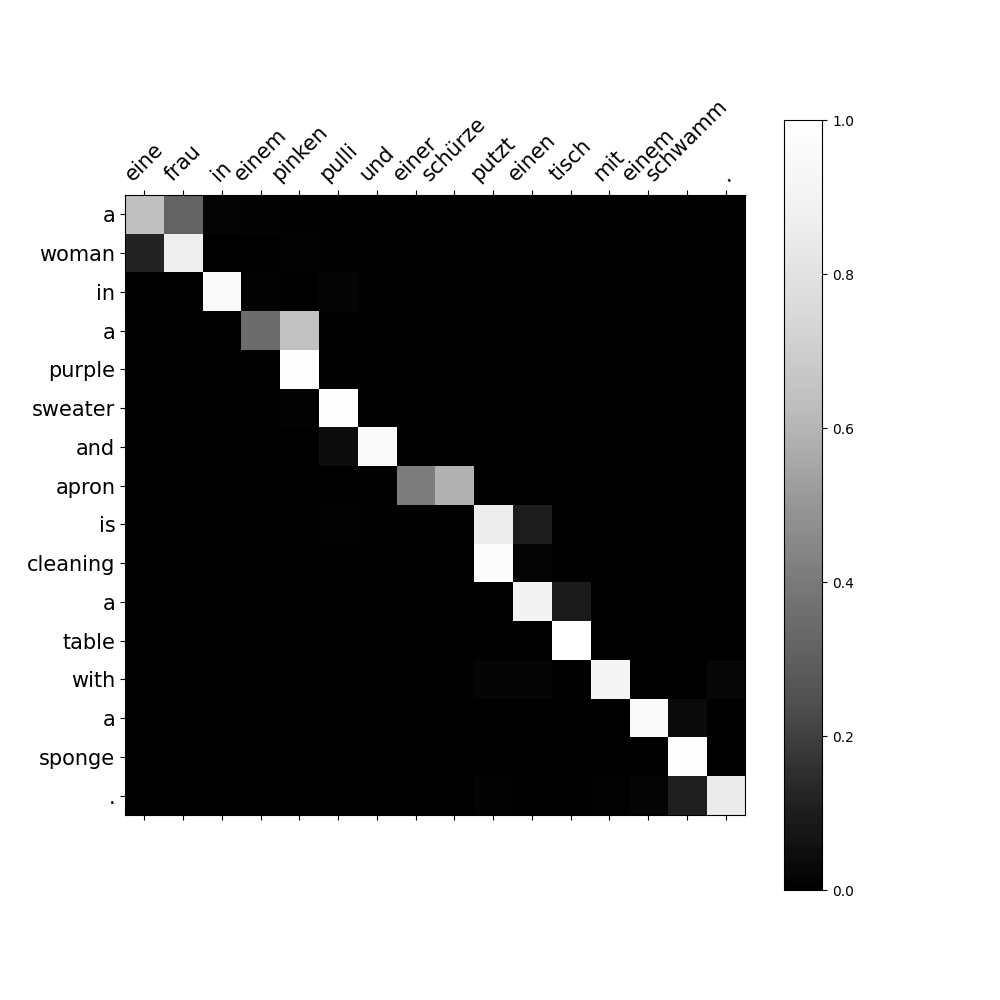
\includegraphics[width=0.8\linewidth]{25_translation.png}
    \caption{Example 1}
\end{figure}

\textbf{Example 1}: This diagram shows a clear alignment between the source and target sentences. The attention focuses on specific pairs of words, shows a direct translation.

\begin{figure}[H]
    \centering
    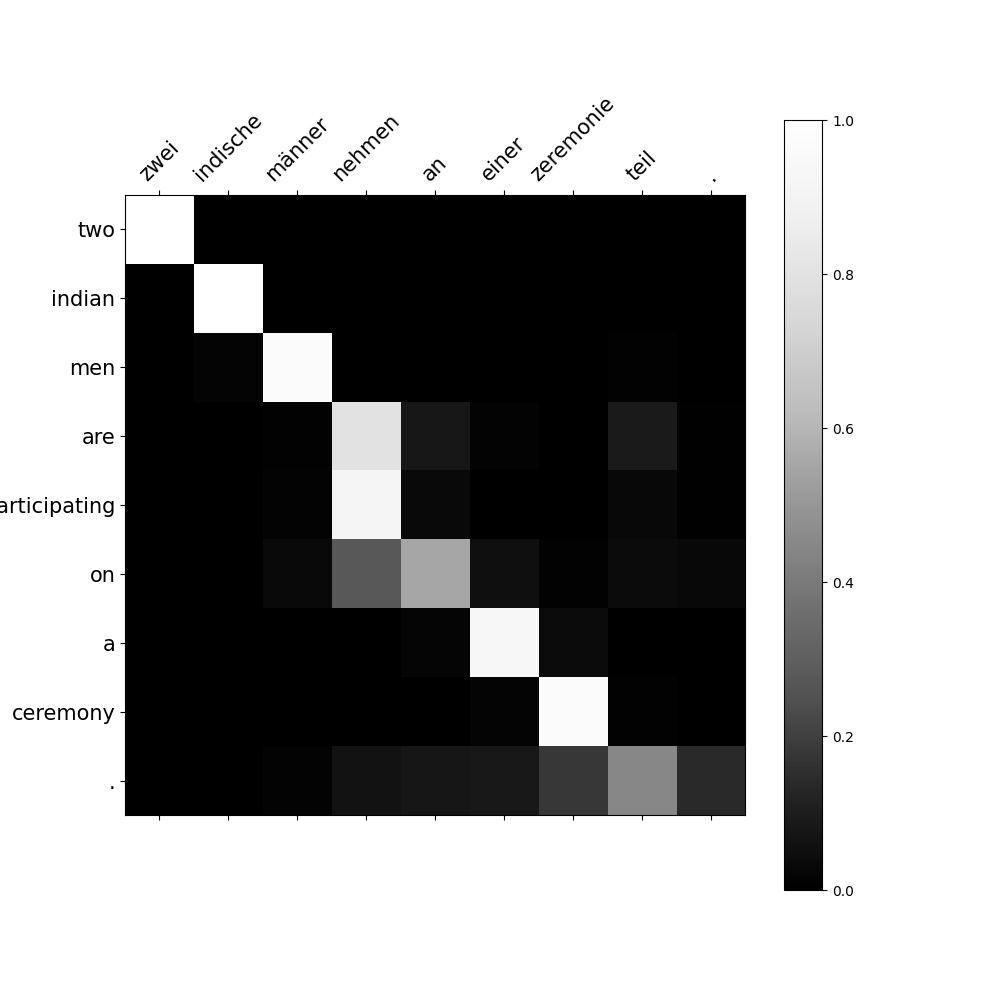
\includegraphics[width=0.8\linewidth]{114_translation.png}
    \caption{Example 2}
\end{figure}


\textbf{Example 2}: This example illustrates how the model handles multiple objects in a sentence, with attention spread across relevant words.

\begin{figure}[H]
    \centering
    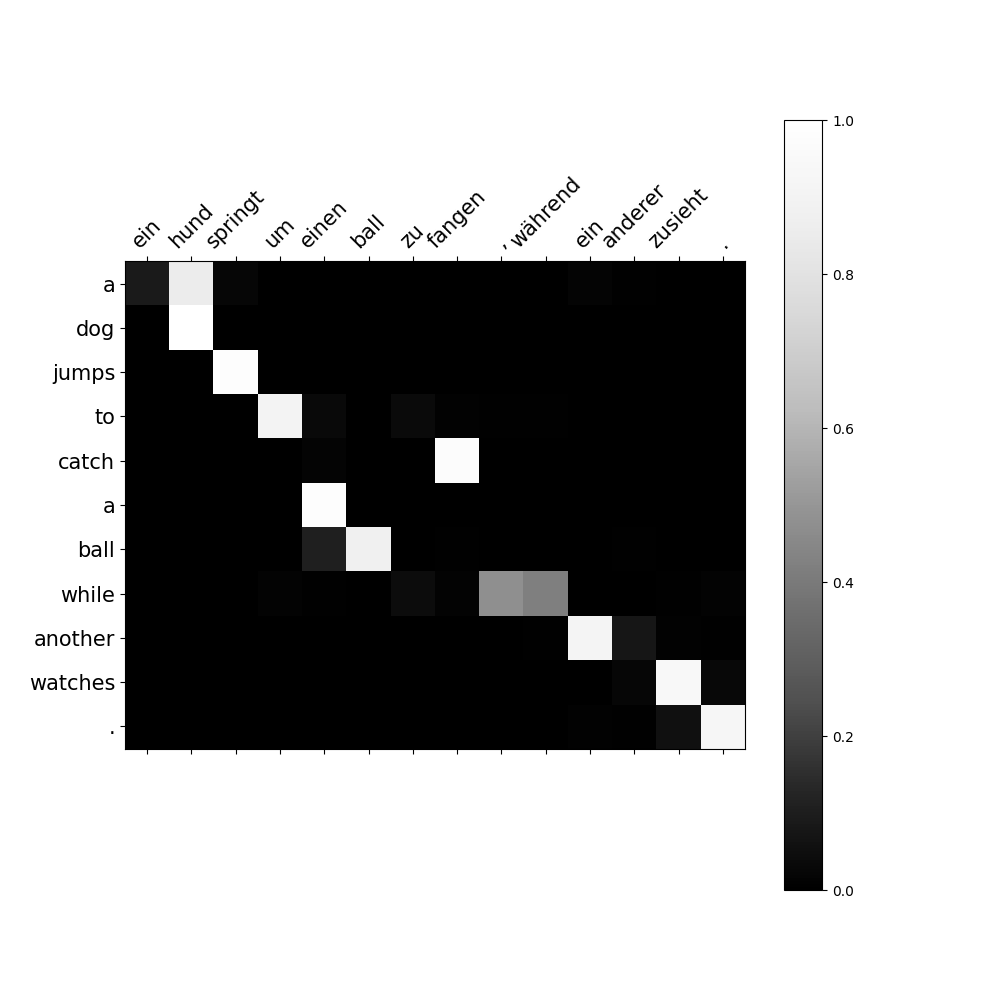
\includegraphics[width=0.8\linewidth]{281_translation.png}
    \caption{Example 3}
\end{figure}


\textbf{Example 3}: The model correctly aligns prepositions and their corresponding objects, showcasing the handling of syntactic structures.

\begin{figure}[H]
    \centering
    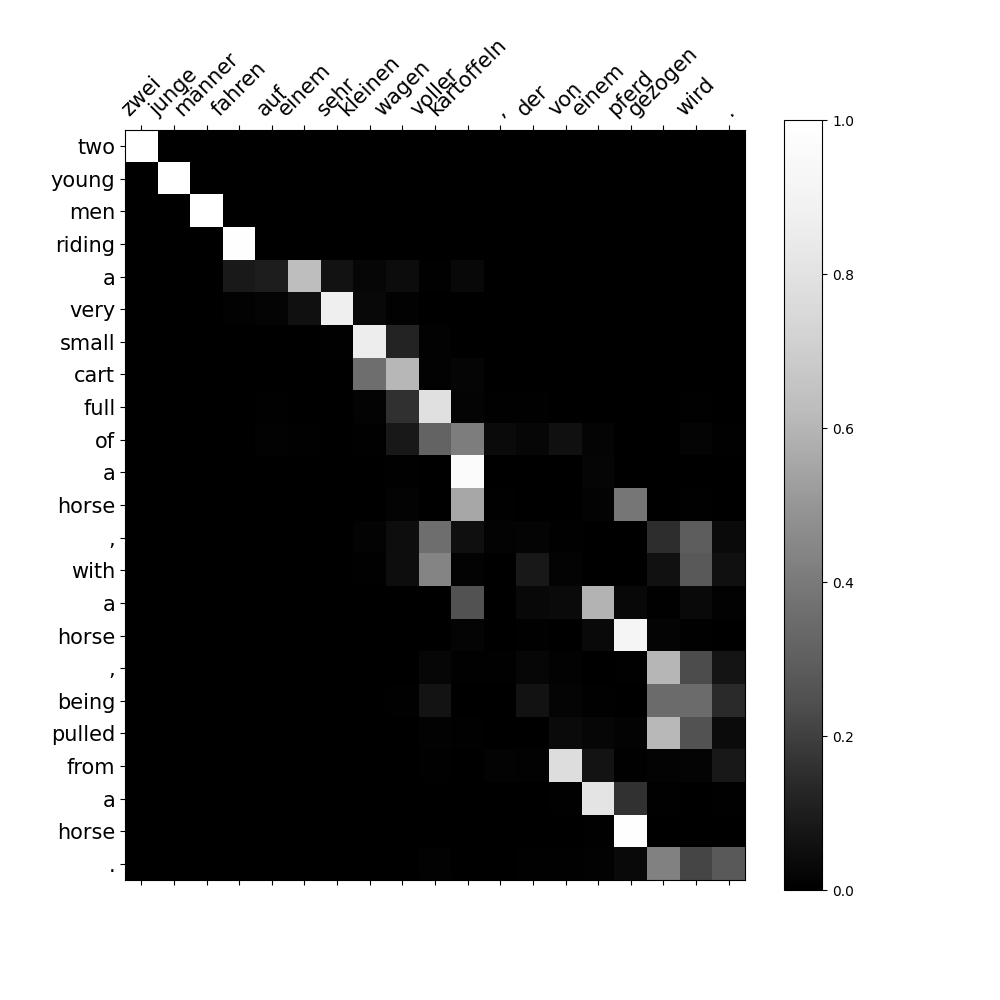
\includegraphics[width=0.8\linewidth]{654_translation.png}
    \caption{Example 4}
\end{figure}


\textbf{Example 4}: Attention is spread across several words, showing the model's capability to handle complex sentence structures.

\begin{figure}[H]
    \centering
    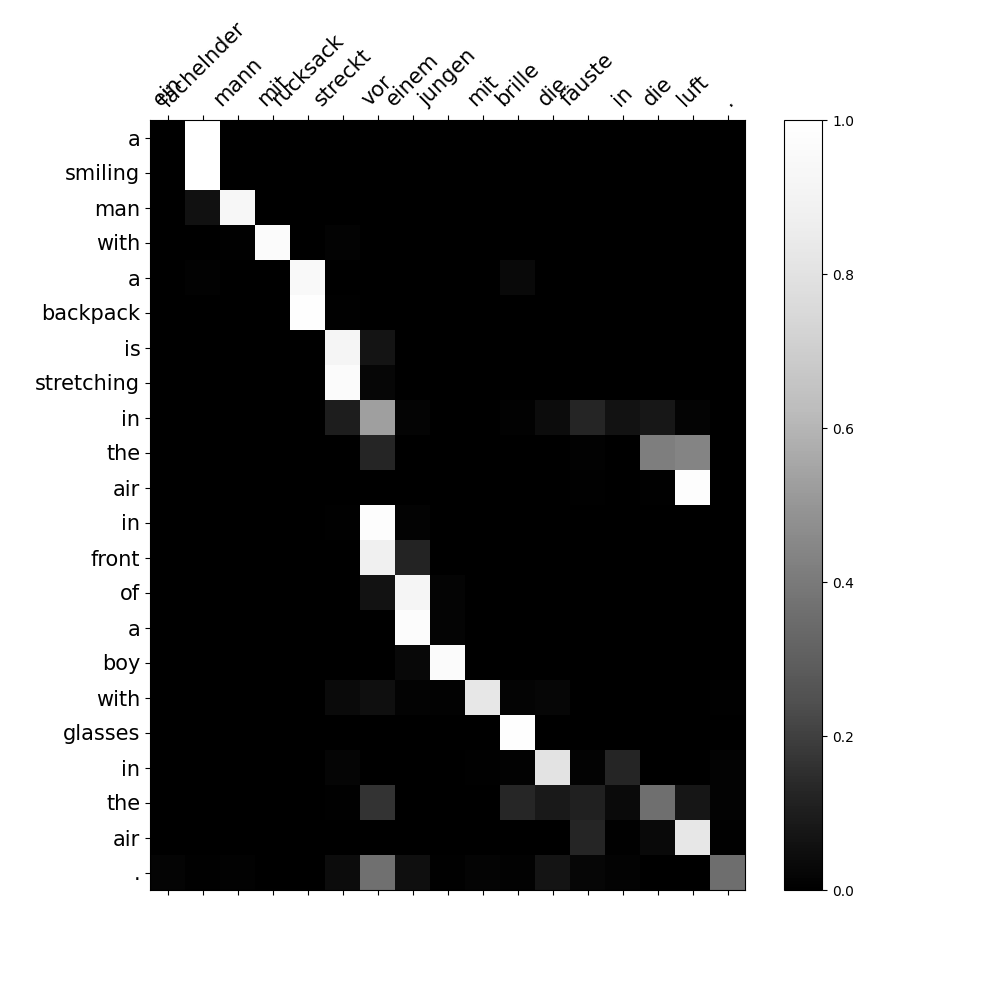
\includegraphics[width=0.8\linewidth]{759_translation.png}
    \caption{Example 8}
\end{figure}
\textbf{Example 5}: The attention focuses on key nouns and verbs, ensuring accurate translation of the main sentence components.
\pagebreak
\subsection{Task 2.3}

\begin{figure}[H]
    \centering
    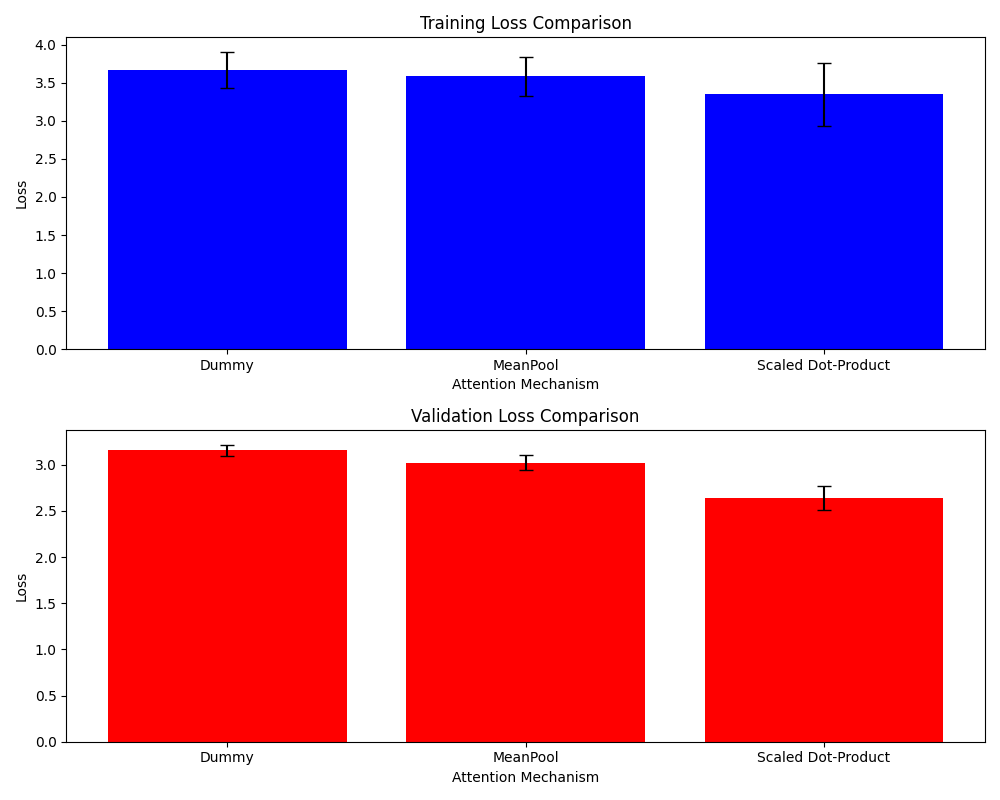
\includegraphics[width=1.0\linewidth]{compare.png}
    \caption{Comparing different attention mechanisms}
    \label{fig:enter-label}
\end{figure}
\textbf{Training Loss Comparison:}

From the training loss plot, we observe the following:
\begin{itemize}
    \item \textbf{Dummy Attention:}
    \begin{itemize}
        \item Mean Training Loss: Approximately 3.67
        \item Variance: 0.232
    \end{itemize}
    \item \textbf{MeanPool Attention:}
    \begin{itemize}
        \item Mean Training Loss: Approximately 3.58
        \item Variance: 0.259
    \end{itemize}
    \item \textbf{Scaled Dot-Product Attention:}
    \begin{itemize}
        \item Mean Training Loss: Approximately 3.35
        \item Variance: 0.411
    \end{itemize}
\end{itemize}

\textbf{Validation Loss Comparison:}

From the validation loss plot, we observe the following:
\begin{itemize}
    \item \textbf{Dummy Attention:}
    \begin{itemize}
        \item Mean Validation Loss: Approximately 3.16
        \item Variance: 0.059
    \end{itemize}
    \item \textbf{MeanPool Attention:}
    \begin{itemize}
        \item Mean Validation Loss: Approximately 3.02
        \item Variance: 0.081
    \end{itemize}
    \item \textbf{Scaled Dot-Product Attention:}
    \begin{itemize}
        \item Mean Validation Loss: Approximately 2.64
        \item Variance: 0.129
    \end{itemize}
\end{itemize}

\textbf{Observed Trends:}

\begin{itemize}
    \item \textbf{Training Loss:}
    \begin{itemize}
        \item The Scaled Dot-Product attention mechanism shows the lowest mean training loss (3.35) compared to Dummy and MeanPool, shows better training performance.
        \item However, the variance for Scaled Dot-Product is higher (0.411), suggesting more variability in the training process.
    \end{itemize}
    \item \textbf{Validation Loss:}
    \begin{itemize}
        \item The Scaled Dot-Product attention mechanism also shows the lowest mean validation loss (2.64), suggesting better generalization to unseen data.
        \item Similar to training loss, the variance is higher for Scaled Dot-Product (0.129), shows some variability in the validation performance.
    \end{itemize}
    \item \textbf{Comparison between Dummy and MeanPool:}
    \begin{itemize}
        \item Both Dummy and MeanPool show similar mean training losses (3.67 and 3.58, respectively) with relatively low variance.
        \item MeanPool slightly outperforms Dummy when it comes to training and validation losses, showing a modest improvement in performance.
    \end{itemize}
    \item \textbf{Overall Performance:}
    \begin{itemize}
        \item The Scaled Dot-Product attention mechanism consistently outperforms Dummy and MeanPool in both training and validation loss metrics.
        \item The higher variance seen with Scaled Dot-Product shows that while it performs better on average, it may not be stable across different runs.
    \end{itemize}
\end{itemize}

\subsubsection*{Conclusion:}
The Scaled Dot-Product attention mechanism demonstrates better performance in reducing both training and validation losses compared to Dummy and MeanPool attention mechanisms. However, this results in higher variance, showing that the performance can change more between different runs. MeanPool shows a slight improvement over Dummy, but not as good as Scaled Dot-Product.
\end{document}
